\chapter{Low Power, yet Powerful}\label{benchmark}
The ARM-based processors have received great attention for its characteristic of low power consumption and energy efficiency, especially in smart phone and portable device industry, where power consumption is one the most critical specifications. Furthermore, there is trend in server industry to shift to ARM-based architecture in order to cut off the bill of electricity. ARM is also ambitious in this area and about to publicize processors capable of virtualization. When it comes to rural development, power shortage has been forcing researchers and engineers to seek for alternative power sources. Lower power consumption of the equipments implies a bigger potential of surviving severe environment.
Currently, we are exploring the possibilities of two platforms, namely Raspberry Pi and Odroid. The specifications of these two platform can be found in Table X
%TODO specification table
In the following sections, we benchmark a variety of attributes of Odroid and Raspberry Pi. The objective is to clarify the capacity of these two platforms and an optimum form to run the web service. We test every component of a complete Moodle installation to identify the bottleneck of the application. Based on the results, we propose the optimum cluster solution that can be easily scaled out to serve more users.

\section{Processor and Bandwidth Latency}


\section{Benchmark of Web Components}
To test components of a complete Moodle installation, we design a expirement in Figure X. Each part is respectively substituted with either Odroid or Raspberry Pi, and remaining parts are running on a high-end which is much more powerful than these two platforms, in order to put enough siege on the testing target. Furthermore, simulated requests are generated from high-end machine as well.

\section{Web Frontend}
Most of the websites today are powered by Apache due to its long history and abundant extensions. Although Apache relies on a processed-based manner to handle new connection, which has limited the scalability and concurrency. Nginx is an event-based reverse proxy that handles request asynchronizily. It addresses C10K problem from the beginning and focus on scalability.
To determine which server runs better on a resource constraint platform, we benchmark Nginx and Apache on both platform to evaluate the throughput, level of concurrency and response delay. We use siege to generate workload and compare the performance of web server with two different type of object: small text file and large JPG file.
We siege the server in following setting:
%TODO topology

\begin{figure}[h]
\centering
\begin{subfigure}{0.45\textwidth}
\centering
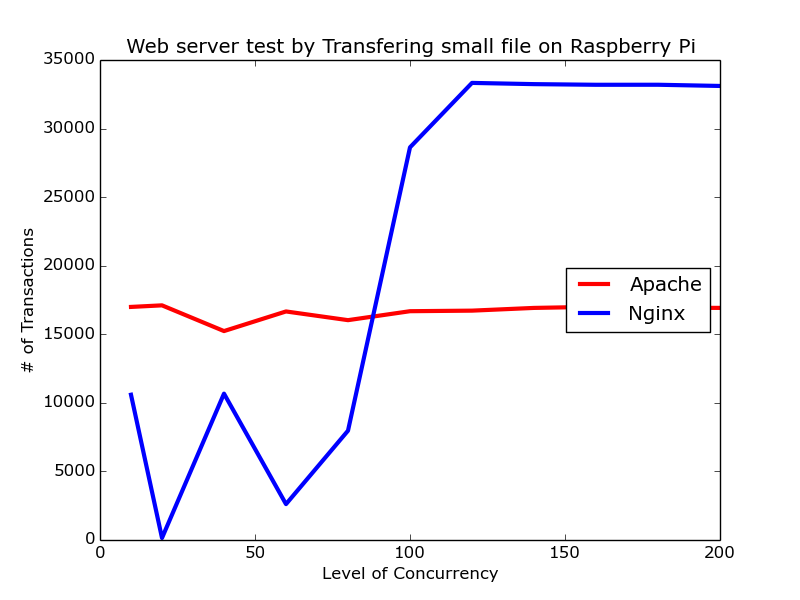
\includegraphics[width=\textwidth]{rpi_small_text.png}
\caption{Raspberry Pi (small text file)}
\end{subfigure}
\begin{subfigure}{0.45\textwidth}
\centering
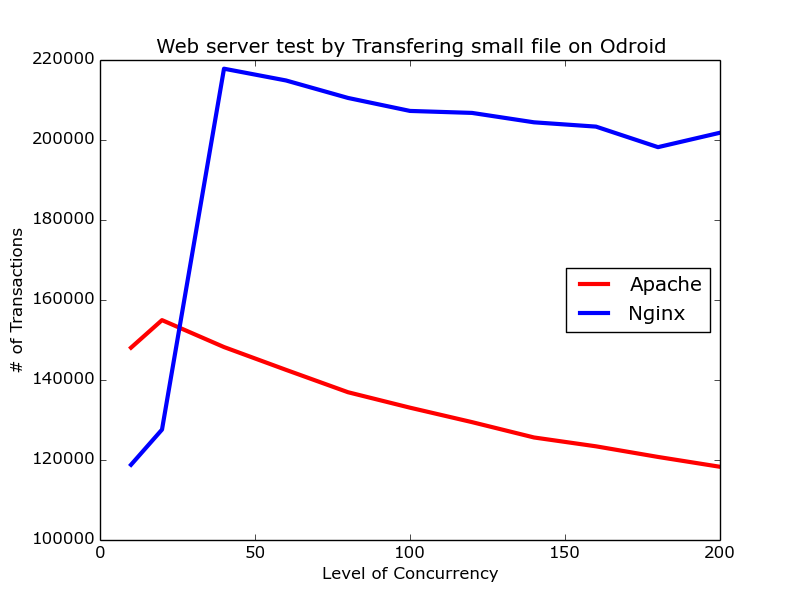
\includegraphics[width=\textwidth]{odroid_small_text.png}
\caption{Odroid (small text file)}
\end{subfigure}

\begin{subfigure}{0.45\textwidth}
\centering
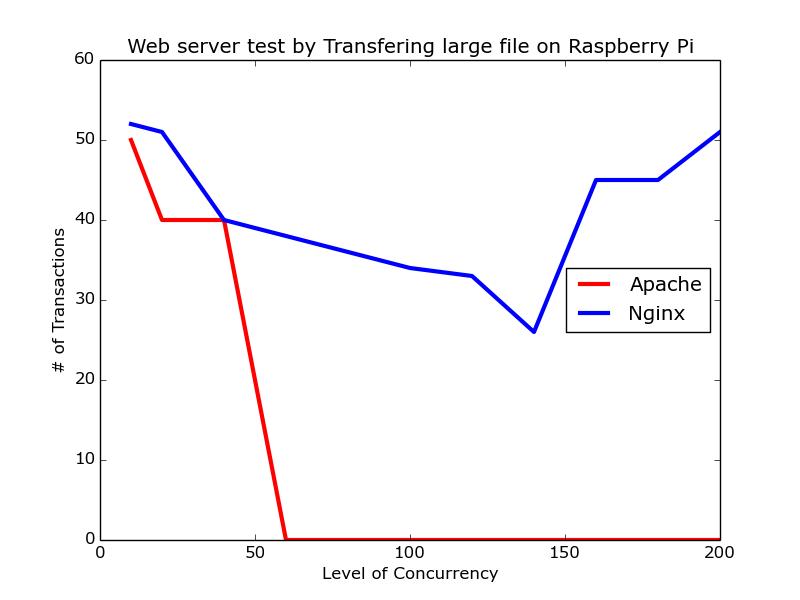
\includegraphics[width=\textwidth]{rpi_big_jpg.png}
\caption{Raspberry Pi (big jpg file)}
\end{subfigure}
\begin{subfigure}{0.45\textwidth}
\centering
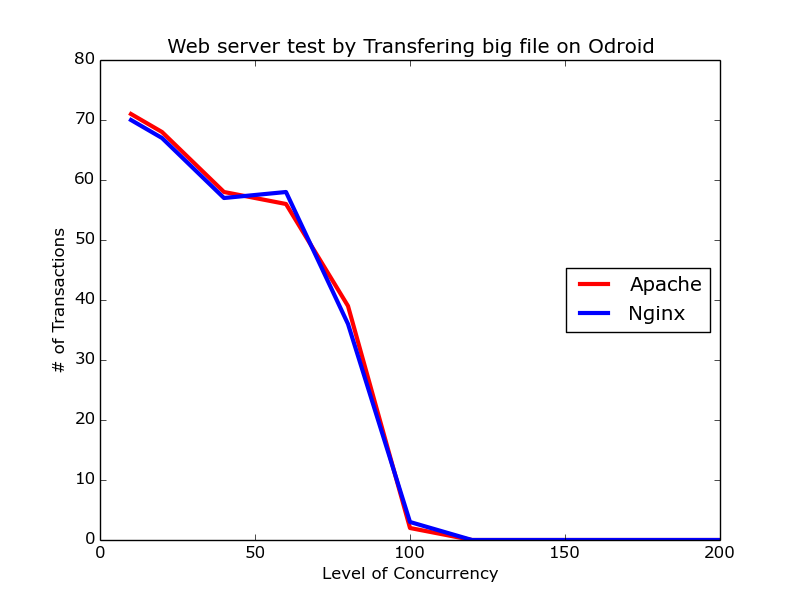
\includegraphics[width=\textwidth]{odroid_big_jpg.png}
\caption{Odroid (big jpg file)}
\end{subfigure}

\caption{A Benchmark of static file request on both platforms}
\label{static}
\end{figure}
%TODO figure
As shown if Figure \ref{static}, Nginx outperforms Apache in concurrency level, transaction per second and availability.

\section{PHP Processing}
As a heavy PHP application, Moodle requires significant computational resources for PHP processing. Thus, a testbed is formed to benchmark processing power of two platforms, see Figure X
%TODO PHP benchmark testbed
The inputs are two different PHP scripts:
\begin{itemize}
\item a php script simply echoes \texttt{Hello, world!}
\item Moodle index page which requires heavy php processing.\footnote{We observe a 6~7 seconds delay to process index page of Moodle on Raspberry Pi and it can barely tolerate the mildest siege. Thus, the test result of Raspberry Pi is left out in this test.}
\end{itemize}

\begin{figure}[h]
\centering
\begin{subfigure}{0.45\textwidth}
\centering
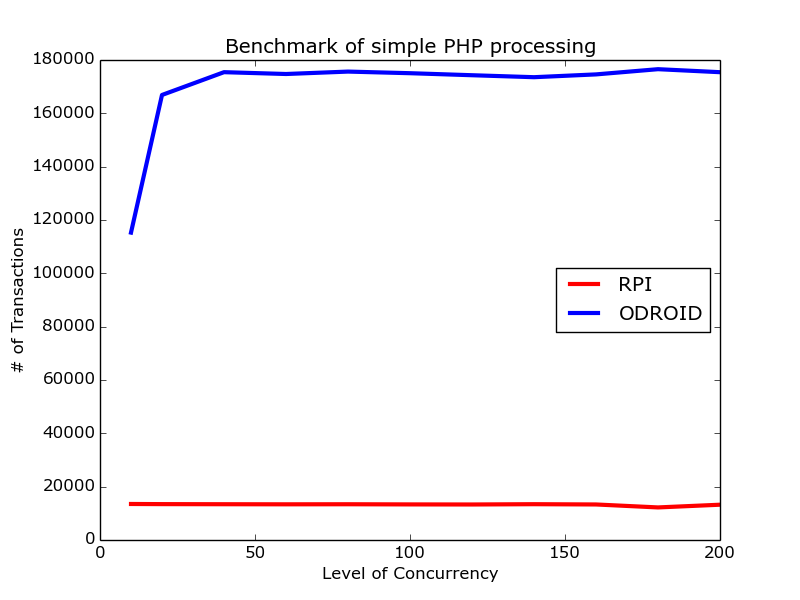
\includegraphics[width=\textwidth]{simple_php.png}
\caption{$\sum trans$}
\end{subfigure}
\begin{subfigure}{0.45\textwidth}
\centering
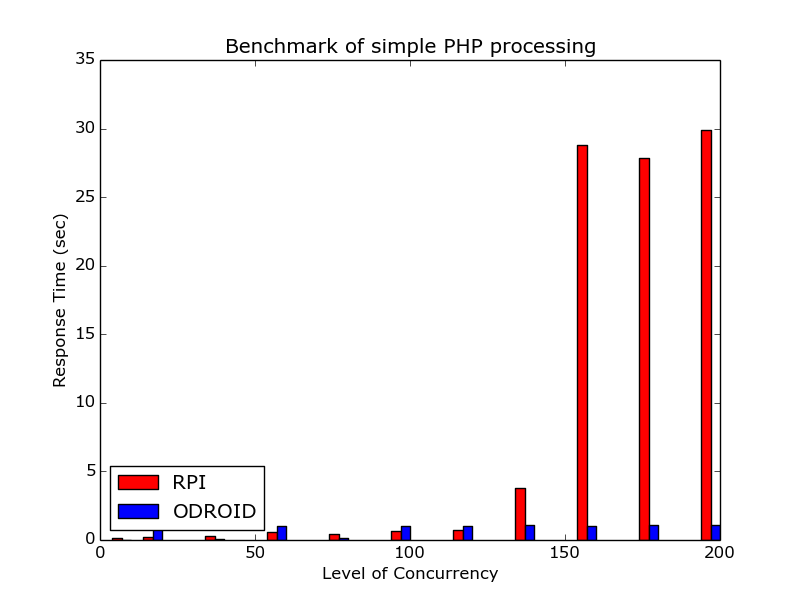
\includegraphics[width=\textwidth]{simple_php_max_res.png}
\caption{Longest Response Time}
\end{subfigure}
\caption{A Benchmark of simple PHP processing on both platforms}
\label{simple_php}
\end{figure}

\begin{figure}[h]
\centering
\begin{subfigure}{0.45\textwidth}
\centering
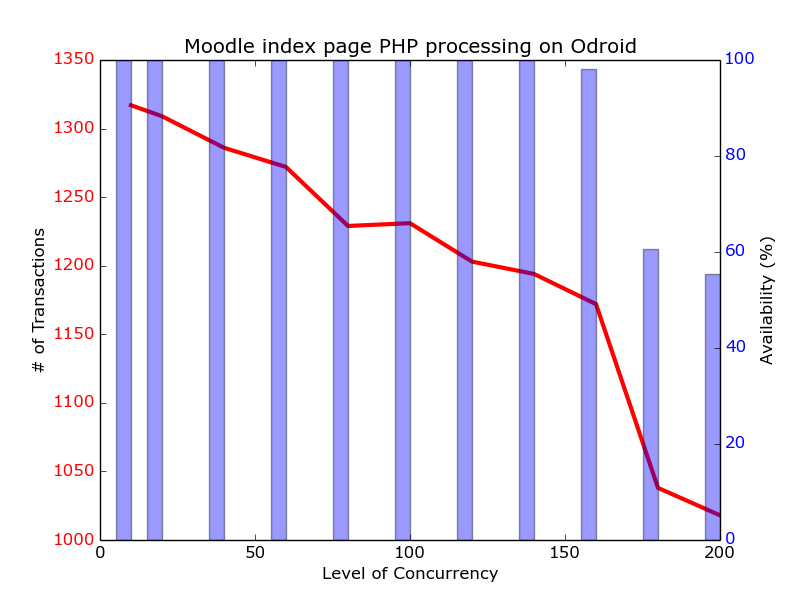
\includegraphics[width=\textwidth]{moodle_index.png}
\caption{$\sum trans$ \& Availability}
\end{subfigure}
\begin{subfigure}{0.45\textwidth}
\centering
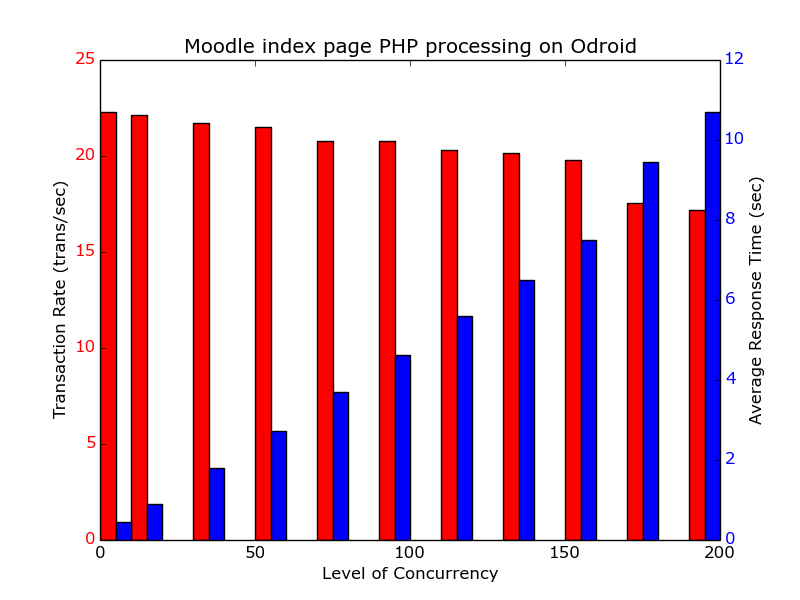
\includegraphics[width=\textwidth]{moodle_index_2.png}
\caption{$Rate_{trans}$ \& $T_{resp}$}
\end{subfigure}
\caption{Moodle index processing on Odroid}
\label{moodle_php_result}
\end{figure}

From the result in Figure \ref{moodle_php_result}, we could clearly understand that Odroid significantly outperforms Raspberry Pi. When Odroid is utilized as a dedicated PHP server, 

\section{Database}

\section{Sale Out to Eliminate Bottleneck}
In third test, we run complete Moodle application on single platform with different front-end web server. We found out that there is no significant difference between two tests. Neglectable impact of web server frontend implies a bottleneck of PHP processing. Thus, we propose a cluster in Figure X where the PHP server can be easily scaled out by adding more hardware.

